\documentclass[conference]{IEEEtran}

% ---------------------------------------------------------------
% Packages
% ---------------------------------------------------------------
\usepackage{cite}
\usepackage{amsmath,amssymb}
\usepackage{booktabs}
\usepackage{graphicx}
\usepackage{xcolor}
\usepackage{url}
\usepackage{microtype}
\usepackage{multirow}
\usepackage{array}
\usepackage{balance}   % balance last-page columns
\usepackage{tikz}
\usetikzlibrary{arrows.meta,positioning,shapes.geometric}

% ---------------------------------------------------------------
% Document
% ---------------------------------------------------------------
\begin{document}

\title{Assurance-Aware Design Space Exploration\\
for Zero-Trust Avionics SoC Security}

% Double-blind submission
\author{\IEEEauthorblockN{[Author names omitted for double-blind review]}}

\maketitle

% ---------------------------------------------------------------
\begin{abstract}
Modern avionics increasingly consolidate safety-critical and
security-sensitive functions onto shared System-on-Chip (SoC) platforms.
This hardware consolidation creates new attack surfaces where a compromised
IP core can reach safety-critical assets through shared bus interconnects.
We present an automated design space exploration (DSE) workflow that
synthesizes zero-trust security architectures for avionics SoCs.
Using Answer Set Programming (ASP), the tool takes a single architectural
model and produces three deliverables: (1)~optimal security feature
assignments under FPGA resource and power constraints with solver-verified
optimality, (2)~least-privilege access control policies with lifecycle mode
awareness, and (3)~resilience checklists derived from automated fault and
compromise scenarios.
The workflow employs an additive risk model aligned with NIST SP~800-30
that separately budgets security risk and availability risk, enabling
independent optimization of feature selection and redundancy architecture.
We evaluate the approach on two case studies: an 8-component SoC drone
and an 11-component UAV translated from the DARPA CASE surveillance
architecture. The tool identifies 9 excess privileges, 6 trust anchor
gaps, and a 3.0$\times$ risk reduction from zero-trust overlay on the SoC
drone, while revealing single-string architecture vulnerabilities in the
UAV that the manual AADL-based approach of Hasan et~al.\ did not surface.
\end{abstract}

\begin{IEEEkeywords}
Zero-Trust Architecture, System-on-Chip Security, Design Space
Exploration, Answer Set Programming, Avionics, DO-326A
\end{IEEEkeywords}

% ---------------------------------------------------------------
\section{Introduction}

The avionics industry is undergoing a fundamental shift toward hardware
consolidation, where multiple safety-critical and security-sensitive
functions are integrated onto shared System-on-Chip (SoC) platforms.
This trend, driven by size, weight, and power (SWaP) optimization, creates
new cybersecurity challenges: a compromised IP core on a shared bus fabric
can potentially access every other component on the same interconnect,
bypassing the physical isolation that traditional federated architectures
provided.

Zero-Trust Architecture (ZTA), as defined by NIST SP~800-207~\cite{nist_zta},
eliminates implicit trust based on network location. The FAA has mandated
ZTA transition for its ground infrastructure~\cite{faa_zt}, and recent work
has called for extending ZTA principles to airborne avionics
systems~\cite{ztas_dasc}. However, applying ZTA to SoC interconnects presents
unique challenges not addressed by enterprise network ZTA: hardware resource
constraints (LUTs, flip-flops, power), real-time requirements, and
the need to co-optimize security feature selection with firewall placement
and access control policy synthesis.

This paper presents an automated DSE workflow that addresses these challenges
through ASP. Given a single SoC architectural model, the tool produces
three deliverables:

\begin{enumerate}
\item \textbf{Optimal security architectures} --- security and logging
  feature assignments minimizing residual risk under FPGA resource and
  power constraints, with solver-verified optimality.
\item \textbf{Access control policies} --- least-privilege ACLs with
  role-based access control, mission-phase awareness (operational,
  maintenance, emergency), and three-mode security policies
  (normal, attack suspected, attack confirmed).
\item \textbf{Resilience checklists} --- automatically generated fault and
  compromise scenarios with quantitative blast radius, service availability,
  capability assessment, and attack path analysis.
\end{enumerate}

The key contributions are:
\begin{itemize}
\item An additive risk model with dual-risk budget separating security risk
  from availability risk, aligned with NIST~SP~800-30 and avoiding
  multiplicative artefacts on ordinal scales.
\item Automated ZTA policy synthesis that co-optimizes firewall topology
  with mode-aware access control, proving infeasibility when constraints
  conflict.
\item Topology-agnostic resilience analysis with firewall-aware blast radius
  and multi-hop attack path enumeration.
\item Evaluation on two case studies demonstrating generality, including a
  comparison with the Collins Aerospace manual ZT pattern approach on
  the same UAV system.
\end{itemize}

% ---------------------------------------------------------------
\section{Related Work}

\textbf{SoC Hardware Security.}
Hardware-enforced isolation on SoCs is well-established through ARM
TrustZone~\cite{arm_tz}, Xilinx isolation design flow~\cite{xilinx_idf},
and secure interconnect architectures~\cite{fiorin_noc}. These provide
static partitioning but do not automatically select or optimize security
feature placement under resource constraints.

\textbf{Avionics Security and ZTA.}
Avionics security is governed by DO-326A~\cite{do326a} for airworthiness
security processes and ARINC~653~\cite{arinc653} for temporal/spatial
partitioning. NIST SP~800-207~\cite{nist_zta} defines zero-trust
principles; the FAA has mandated ZTA transition for ground
infrastructure~\cite{faa_zt}. Hasan et~al.~\cite{hasan_saecps,hasan_jsys}
defined AADL-based ZT architecture patterns for cyber-physical systems and
demonstrated manual application to a UAV surveillance system. Their stated
future work is to ``build a tool that provides the ability to leverage ZT
architecture patterns and build ZT compliant CPS systems while providing
design-time assurance.'' This paper addresses that objective through
constraint solving. The DARPA CASE program~\cite{darpa_case} produced
the BriefCASE toolchain for AADL model transformations with
CakeML-verified components on seL4. A 2023 DASC paper~\cite{ztas_dasc}
called for simultaneous functionality-security co-design in avionics.

\textbf{Risk Quantification and DSE.}
CVSS~\cite{cvss} and NIST SP~800-30~\cite{nist_sp80030} provide risk
frameworks. Aven~\cite{aven_riskmatrix} identified artefacts in
multiplicative risk matrices on ordinal scales; our additive model avoids
these. Heuristic approaches (NSGA-II, genetic algorithms) cannot prove
optimality; ASP provides exact solutions with constraint satisfaction
guarantees~\cite{gebser_asp}.

\textbf{Positioning.}
Unlike Collins' manual pattern application, our ASP formulation explores the
full design space and verifies optimality. Unlike BriefCASE's model
transformations, we simultaneously synthesize feature assignments, firewall
placement, and access policies under quantitative resource constraints.

% ---------------------------------------------------------------
\section{System Model and Threat Model}

\subsection{SoC Graph Model}
We model the SoC as a directed graph $G=(V,E)$ where vertices are typed:
$V_M$~(bus masters), $V_R$~(receiver IP cores), $V_B$~(bus
interconnects), $V_{FW}$~(Policy Enforcement Points), $V_{PS}$~(Policy
Decision Points). Each component is annotated with trust domain, CIA impact,
and exploitability (Table~\ref{tab:features}).

\subsection{Threat Model}
We consider an attacker who can compromise any single component or bus,
with effects propagating through the interconnect topology:
\begin{itemize}
\item \textit{Direct compromise}: attacker controls a component's assets.
\item \textit{Cross-domain escalation}: compromised low-trust component
  reaches high-trust assets.
\item \textit{Control plane attack}: policy server compromise bypasses all
  governed firewalls.
\item \textit{Common-mode failure}: shared bus failure cuts off all
  connected components.
\end{itemize}

\subsection{Security Features}
Each receiver is assigned one security feature and one logging feature from
a catalog with Vivado post-implementation resource estimates
(Table~\ref{tab:features}).

\begin{table}[t]
\caption{Security Feature Catalog (PYNQ-Z2 Target)}
\label{tab:features}
\centering
\scriptsize
\begin{tabular}{lrrrr}
\toprule
Feature & LUTs & FFs & mW & Protect \\
\midrule
no\_security     &    0 &    0 &  0 & 0 \\
mac              &  650 &  480 & 12 & 4 \\
dynamic\_mac     & 1200 &  920 & 22 & 5 \\
zero\_trust      & 2100 & 1500 & 38 & 6 \\
\midrule
no\_logging      &    0 &    0 &  0 & 0 \\
some\_logging    &  180 &  140 &  4 & 1 \\
zt\_logger       &  450 &  320 &  8 & 2 \\
\bottomrule
\end{tabular}
\end{table}

% ---------------------------------------------------------------
\section{Workflow and ASP Formulation}

Fig.~\ref{fig:workflow} summarizes the three-phase pipeline.
Each phase is an independent ASP program whose output feeds the next.

\begin{figure}[t]
\centering
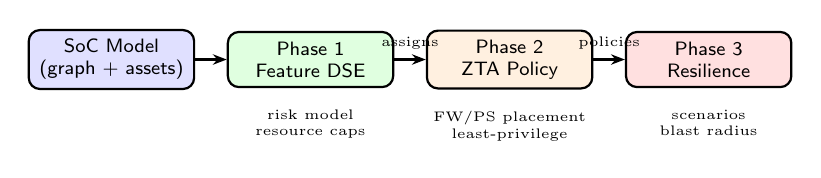
\begin{tikzpicture}[
  node distance=0.4cm,
  box/.style={draw, rounded corners, minimum width=2.1cm,
              minimum height=0.7cm, font=\scriptsize\sffamily,
              align=center, thick},
  arr/.style={-{Stealth[length=5pt]}, thick}
]
\node[box, fill=blue!12]  (input) {SoC Model\\(graph + assets)};
\node[box, fill=green!12, right=of input] (p1) {Phase~1\\Feature DSE};
\node[box, fill=orange!12, right=of p1]   (p2) {Phase~2\\ZTA Policy};
\node[box, fill=red!12, right=of p2]      (p3) {Phase~3\\Resilience};
\draw[arr] (input) -- (p1);
\draw[arr] (p1) -- node[above, font=\tiny] {assigns} (p2);
\draw[arr] (p2) -- node[above, font=\tiny] {policies} (p3);
\node[below=0.15cm of p1, font=\tiny, align=center]
  {risk model\\resource caps};
\node[below=0.15cm of p2, font=\tiny, align=center]
  {FW/PS placement\\least-privilege};
\node[below=0.15cm of p3, font=\tiny, align=center]
  {scenarios\\blast radius};
\end{tikzpicture}
\caption{Three-phase DSE workflow. Phase outputs cascade: security
  assignments feed policy synthesis, which feeds resilience analysis.}
\label{fig:workflow}
\end{figure}

\subsection{Phase~1: Security Feature DSE}

\textbf{Risk Model.} For each component $c$ with asset $a$ and action
$\mathit{op} \in \{\mathit{read},\mathit{write},\mathit{avail}\}$:
\begin{equation}
R(c,a,\mathit{op}) = \max\!\bigl(0,\;\mathit{Imp}+\mathit{DB}+\mathit{EM}
  -\mathit{EP}-\mathit{LP}\bigr)
\label{eq:risk}
\end{equation}
where $\mathit{Imp}$ is CIA impact, $\mathit{DB} \in [0,3]$ maps trust
domains to bonus (low$\to$3, normal$\to$0), $\mathit{EM} =
\mathit{exploitability} - 3 \in [-2,+2]$ offsets from the median CVSS~v3.1
attack complexity for SoC IP cores, $\mathit{EP}$ dispatches to security
(read/write) or availability (avail) protection tables, and $\mathit{LP}$
is the logging detection capability.

The solver assigns exactly one security feature and one logging feature per
component, then minimizes the sum of weighted risk across all
$(c, a, \mathit{op})$ triples subject to resource and risk cap constraints.

\textbf{Dual-Risk Budget.} Two independent hard constraints replace a single
risk cap:
\begin{enumerate}
\item \textit{Security risk budget}: $R(c,a,\mathit{op}) \le
  \mathit{Cap}_\mathit{sec}$ for non-redundant components.
\item \textit{Availability risk budget}: $\mathit{Imp} \times
  P_\mathit{combined} / 100 \le \mathit{Cap}_\mathit{avail}$ for redundant
  group members, where $P_\mathit{combined} = \prod p_i \times 10^k$,
  scaled to $[0,100]$.
\end{enumerate}

\subsection{Phase~2: ZTA Policy Synthesis}

Phase~2 synthesizes firewall and policy server placement with cost
minimization subject to isolation constraints: every low-trust master that
can topologically reach a critical IP must be mediated by a firewall.
Least-privilege analysis compares topology-implied access against declared
needs, flagging $\mathit{excess\_privilege}(M,C,\mathit{Op})$ for every
grant not in $\mathit{access\_need}$.

\textbf{Mode-aware access control} operates in three security modes:
\textit{normal} (role-based access per declared needs);
\textit{attack\_suspected} (only attested masters access non-critical IPs);
\textit{attack\_confirmed} (full isolation of all IPs).
Trust anchor gap detection identifies components lacking hardware root of
trust, secure boot, attestation, or key storage.

\subsection{Phase~3: Resilience Analysis}

Scenarios are auto-generated from the topology, covering single-master
compromise, bus failures, PS/PEP compromise, redundancy group attacks,
combined fault$+$compromise scenarios, and control plane degradation.
For each scenario the solver computes blast radius (structural and
firewall-aware), service availability, capability assessment,
attack paths ($\le$5~hops), and risk amplification factors.

% ---------------------------------------------------------------
\section{Implementation}

The tool is implemented in Python~3.12 with the Clingo~5.8 ASP solver
(13,701 lines across 33 files: 15 ASP encodings, 8 Python core modules,
4 phase orchestrators, 5 GUI modules, and 1 Vivado IP catalog).
The IP catalog provides Xilinx Zynq-7000 (PYNQ-Z2, xc7z020clg400-1)
post-implementation resource estimates.
Phase solve times: Phase~1 $<$5~s (TC9) / 15.5~s (UAV max\_security);
Phase~2 $<$2~s; Phase~3 $<$30~s for 18--24 scenarios.
UAV min\_resources requires progressive-timeout continuation (63~min) to
prove optimality. The orchestrator runs three
optimization strategies in parallel: max\_security, min\_resources, and
balanced. Input modes include built-in factory models and a drag-and-drop
network editor with JSON save/load and ASP export. The tool is available
as open-source software [URL redacted for double-blind review].

% ---------------------------------------------------------------
\section{Case Studies and Results}

\begin{figure}[t]
  \centering
  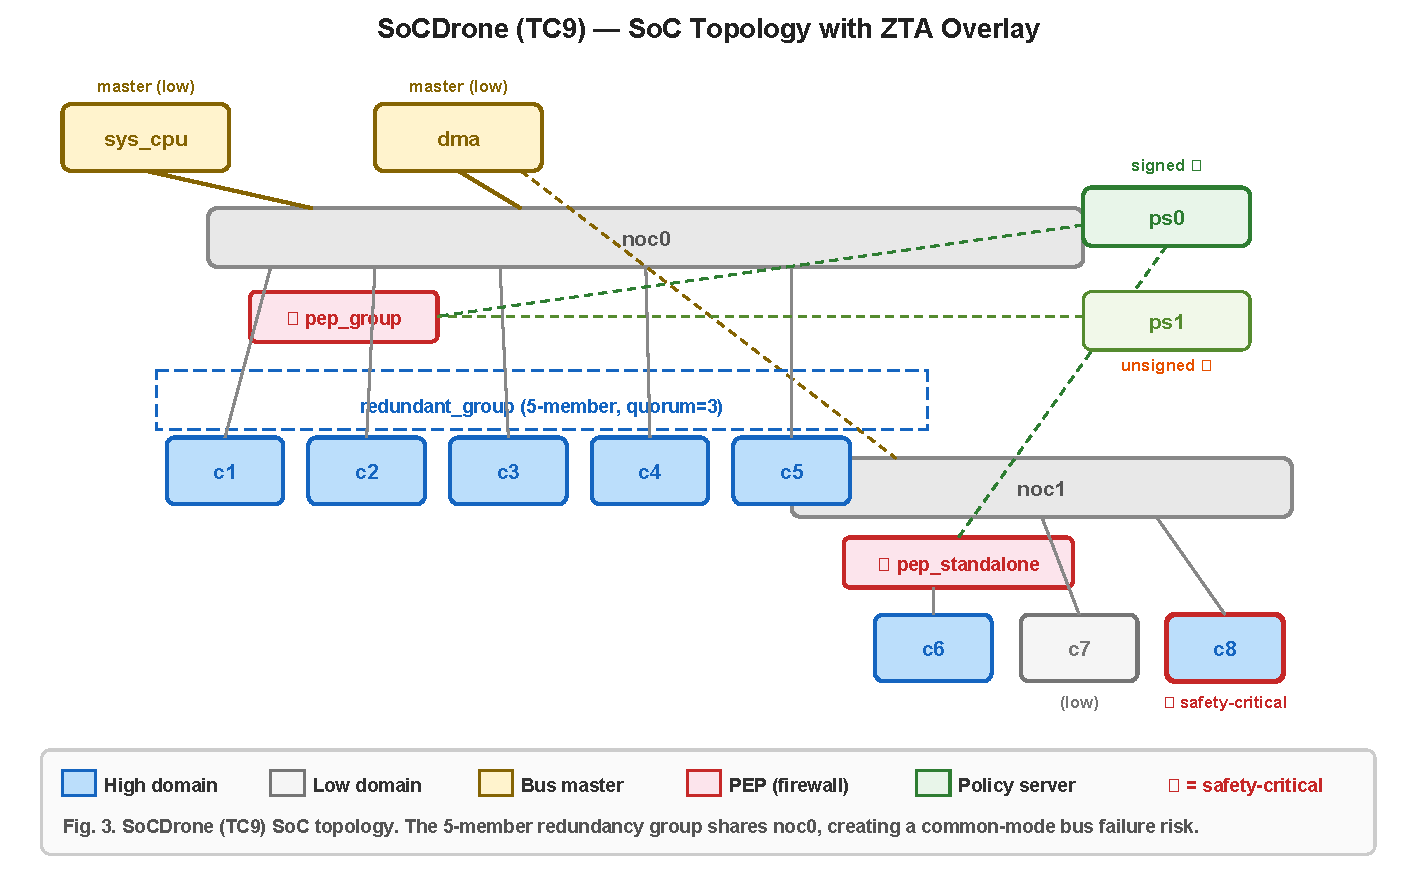
\includegraphics[width=\columnwidth]{fig3_tc9_topology}
  \caption{SoCDrone (TC9) SoC topology. The 5-member redundancy group
    shares noc0, creating a common-mode bus failure risk. pep\_group and
    pep\_standalone are Phase~2 firewall placements.}
  \label{fig:tc9}
\end{figure}

\subsection{Case Study~1: SoCDrone (TC9)}

The SoCDrone is an 8-component SoC with 2 bus masters, 2 NoC buses, a
5-member redundancy group (c1--c5), and 3 standalone IPs including one
safety-critical component (c8).

\textbf{Phase~1 Results.} All three strategies achieve solver-verified
optimality (max\_security in 3.8~s, min\_resources in 8.2~s, balanced in
7.6~s). Under max\_security, total weighted risk is minimized to~74 at
17\% LUTs (9,120/53,200) and 179~mW. Under min\_resources, all components
converge to mac (the minimum-cost feature satisfying the risk cap), cutting
LUT usage to 10\% (5,380/53,200) and power to 100~mW at the cost of raising
weighted risk to~101 --- a 37\% LUT reduction for a 36\% risk increase.
Balanced produces identical assignments to min\_resources for this instance,
indicating that the risk--resource frontier has only two distinct optima
for TC9's 8-component problem.

\begin{table}[t]
\caption{TC9 Phase~1 --- Security Assignments by Strategy}
\label{tab:tc9p1}
\centering
\scriptsize
\setlength{\tabcolsep}{3pt}
\begin{tabular}{lllrllr}
\toprule
 & \multicolumn{2}{c}{max\_security} & & \multicolumn{2}{c}{min\_resources} & \\
\cmidrule(lr){2-3}\cmidrule(lr){5-6}
Comp. & Security+Log & wRisk & & Security+Log & wRisk \\
\midrule
c1 & mac + none         & 14 & & mac + none        & 18 \\
c2 & dyn\_mac + some    & 17 & & mac + none        & 21 \\
c3 & zt + none          & 14 & & mac + none        & 18 \\
c4 & dyn\_mac + none    & 17 & & mac + none        & 21 \\
c5 & mac + zt\_log      & 12 & & mac + none        & 15 \\
c6 & zt + zt\_log       &  0 & & mac + some        &  4 \\
c7 & mac + some         &  0 & & mac + none        &  0 \\
c8 & dyn\_mac + zt\_log &  0 & & mac + none        &  4 \\
\midrule
\textbf{Total} & & \textbf{74} & & & \textbf{101} \\
LUTs / mW & & 9,120 / 179 & & & 5,380 / 100 \\
\bottomrule
\end{tabular}
\end{table}

\begin{table}[t]
\caption{TC9 Multi-Strategy Summary}
\label{tab:tc9strat}
\centering
\scriptsize
\begin{tabular}{lrrr}
\toprule
Metric & max\_sec & min\_res & balanced \\
\midrule
Total weighted risk     &  74 & 101 & 101 \\
LUTs used               & 9,120 & 5,380 & 5,380 \\
Power (mW)              & 179 & 100 & 100 \\
Firewalls placed        &   2 &   2 &   2 \\
Policy servers          &   1 &   1 &   1 \\
Excess privileges       &   9 &   9 &   9 \\
Trust anchor gaps       &   6 &   6 &   6 \\
Worst amplification     & 3.00$\times$ & 3.00$\times$ & 3.00$\times$ \\
Phase~1 solve time (s)  & 3.8 & 8.2 & 7.6 \\
\bottomrule
\end{tabular}
\end{table}

\textbf{Phase~2 Results.} ZTA synthesis placed 2 firewalls (pep\_group,
pep\_standalone) and 1 policy server (ps0). The solver identified 9 excess
privilege grants: the DMA controller has read$+$write access to all IPs but
only needs write to c1--c5 and read to c8 (policy tightness~43\%).
Trust anchor analysis revealed 6 components lacking hardware root of trust,
1 unattested master (dma), and 1 unsigned policy server (ps1).

\textbf{Phase~3 Results.} Eighteen scenarios were executed.
Key findings: (1)~ps0 compromise is the highest-impact single event
(2.5$\times$ risk amplification) because ps0 governs both firewalls;
(2)~noc0 failure is a common-mode failure for all 5 redundancy-group
members simultaneously.

\noindent\fbox{\parbox{\columnwidth}{\scriptsize
\textbf{FINDING-1 (HIGH):} DMA holds 9 excess privilege grants including
write access to safety-critical c8. Policy tightness = 43\%.\\[2pt]
\textbf{FINDING-2 (HIGH):} ps0 compromise bypasses all firewall protection
(2.5$\times$). ps1 lacks signed-policy enforcement.\\[2pt]
\textbf{FINDING-3 (MEDIUM):} noc0 is a common-mode failure for all 5
redundancy-group members. c7's no\_logging creates an unmonitored attack
path.
}}

\begin{figure}[t]
  \centering
  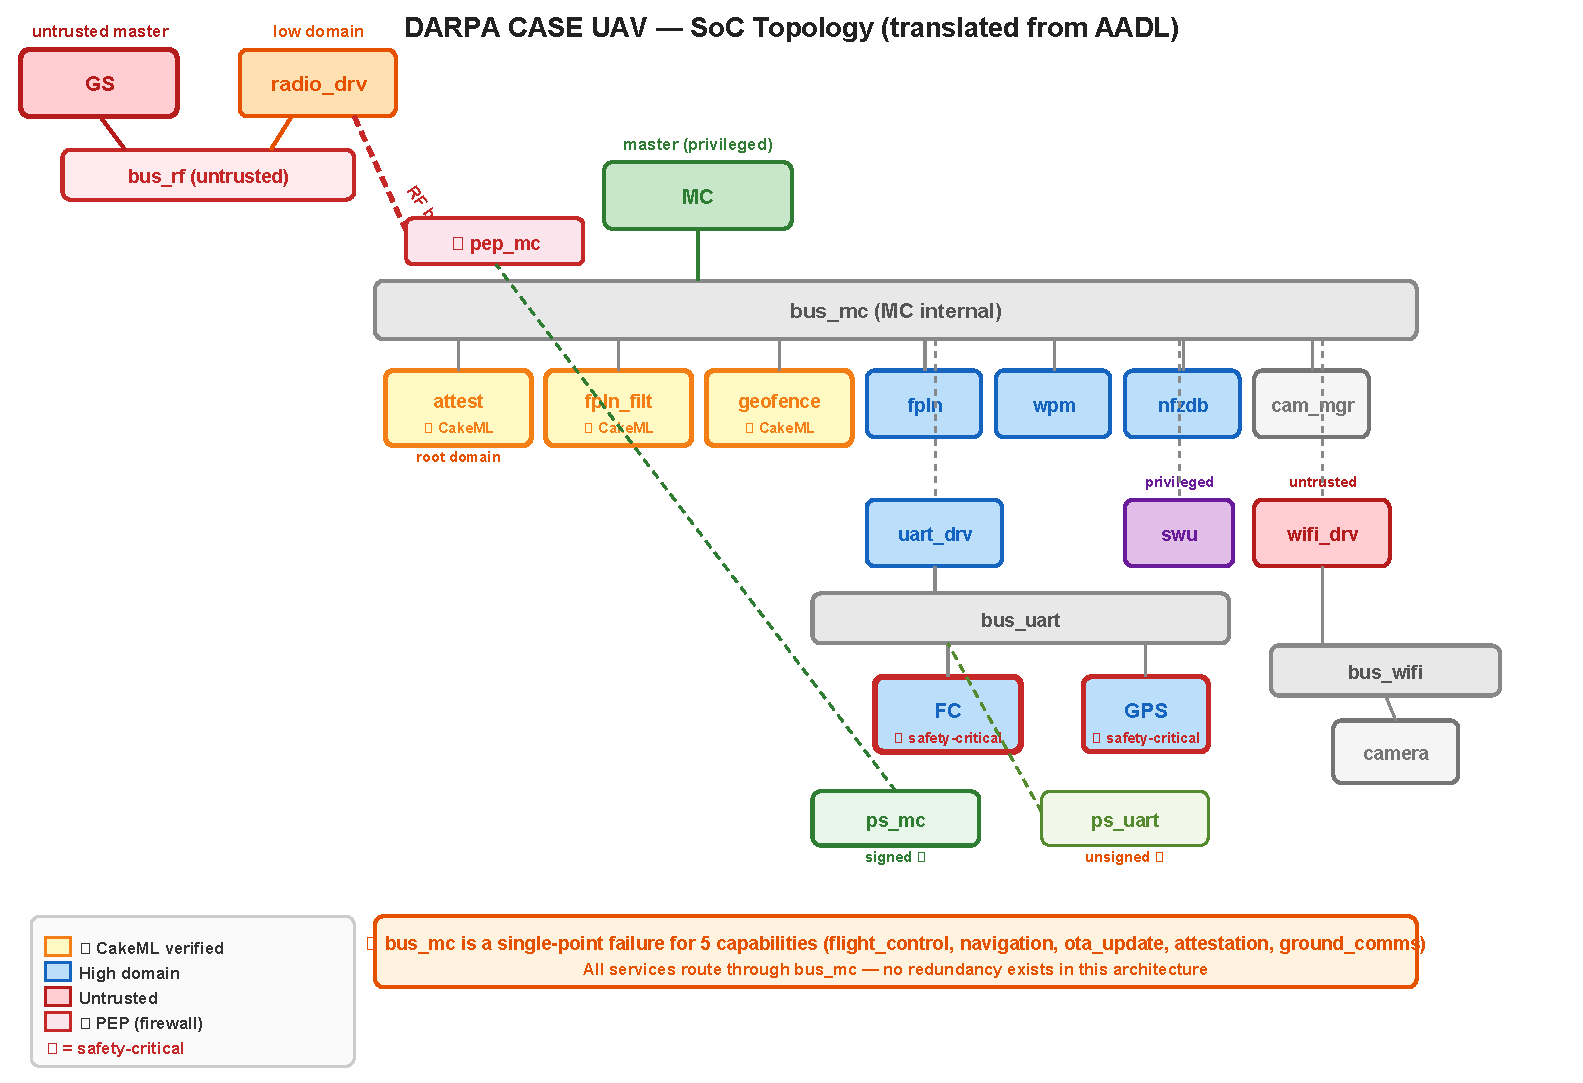
\includegraphics[width=\columnwidth]{fig4_darpa_uav_topology}
  \caption{DARPA CASE UAV SoC topology (translated from AADL).
    radio\_drv bridges the untrusted RF bus into the trusted MC internal
    bus --- the primary attack path. All services route through bus\_mc,
    making it a single-point availability failure.}
  \label{fig:uav}
\end{figure}

\subsection{Case Study~2: DARPA CASE UAV}

We translated the DARPA CASE UAV surveillance architecture --- the same
system used by Hasan et~al.~\cite{hasan_saecps} to demonstrate manual ZT
pattern application --- from its AADL software representation into our SoC
interconnect model. The translated architecture has 11 receivers
across 4 buses, 3 masters, 4 safety-critical components, and zero
redundancy groups, including three BriefCASE/Collins hardening additions
(attestation gate, flight plan filter, geofence monitor, all CakeML-verified).

\textbf{Phase~1.} Under max\_security (proven optimal in 15.5~s),
zero\_trust$+$zt\_logger is assigned to 8 of 11 components, achieving total
risk~=~0 at 34\% LUT utilization (18,170/53,200 LUTs, 367~mW).
CakeML-verified components (exploitability=1) achieve risk=0 without
dominating the resource budget.
Under min\_resources, a progressive-timeout continuation run proved
optimality after 6 attempts totaling 63~minutes (Table~\ref{tab:convergence}).
The proven-optimal solution assigns mac to all 11 components with selective
some\_logging, achieving risk~=~39 at 15\% LUTs (8,410/53,200) and 160~mW
--- a 54\% LUT reduction versus max\_security for a risk increase from 0
to~39.

\textbf{Phase~2.} ZTA synthesis placed 1 firewall (pep\_mc) and 1 policy
server (ps\_uart). The solver identified 22 excess privileges: the ground
station (gs, untrusted) has 10\% policy tightness, holding topological
access to all 9~MC-bus components via the radio\_drv bridge while
requiring only radio\_drv read$+$write. Trust anchor analysis found 10
components lacking RoT, 2 unattested masters (fc, gs), and 1 unsigned
policy server.

\textbf{Phase~3.} Under max\_security all 24 scenario risks are~0 (base
risk~0 $\times$ amplification~=~0). Under min\_resources (baseline
risk~=~42.2), worst-case 2.06$\times$ amplification under ps\_uart
compromise (risk~=~87.0).
Key finding: \texttt{bus\_mc\_failure} loses \textbf{5 capabilities
simultaneously} (flight\_control, navigation, ota\_update, attestation,
ground\_comms) --- a single-point availability failure that no security
feature assignment can mitigate.

\begin{table}[t]
\caption{UAV min\_resources Progressive-Timeout Convergence}
\label{tab:convergence}
\centering
\scriptsize
\begin{tabular}{rrrrrrl}
\toprule
Att. & Timeout & Models & Risk & LUTs & mW & Status \\
\midrule
1 &   60~s & 15 & 31 & 10,240 & 198 & best-found \\
2 &  120~s & 10 & 34 &  9,380 & 180 & best-found \\
3 &  300~s &  4 & 38 &  9,130 & 174 & best-found \\
4 &  600~s &  8 & 39 &  8,410 & 160 & best-found \\
5 & 1200~s &  0 & 39 &  8,410 & 160 & no improvement \\
6 & 1800~s &  0 & 39 &  8,410 & 160 & \textbf{proven optimal} \\
\bottomrule
\end{tabular}
\end{table}

\textbf{Comparison with Manual Hardening.}
Table~\ref{tab:comparison} compares the automated tool with the manual AADL
ZT pattern approach of Hasan et~al.~\cite{hasan_saecps} on the same UAV.
This comparison should be read as portability evidence rather than a strict
``tool versus Hasan'' evaluation: the manual AADL-based work and the present
SoC DSE operate at different abstraction levels (software architecture with
CakeML-verified components on seL4 vs.\ hardware interconnect topology).
The value is that the automated tool exposes privilege and topology findings
that complement, rather than replace, the manual pattern approach.

\begin{table}[t]
\caption{Automated DSE vs.\ Manual AADL Hardening (Same UAV)}
\label{tab:comparison}
\centering
\scriptsize
\setlength{\tabcolsep}{2pt}
\begin{tabular}{lp{14em}p{14em}}
\toprule
Dimension & Collins Manual~\cite{hasan_saecps} & This Tool \\
\midrule
Scope     & SW architecture (AADL) & HW interconnect (SoC) \\
Method    & Manual pattern selection & Constraint-solving DSE \\
Space     & Designer's choice & All $3^{11}$ combos \\
Optimality& None & Solver-verified (both strategies) \\
Privilege & Not in scope & 22 excess flagged \\
Trust gaps& Not in scope & 10 no-RoT, 2 unattested \\
Modes     & 1 (hardened) & 9 (3$\times$3) \\
Resilience& Not in scope & 24 scenarios \\
SPOF      & Not in scope & bus\_mc: 5-cap failure \\
Resources & Not in scope & 34\% LUT (max); 15\% (min) \\
\bottomrule
\end{tabular}
\end{table}

\subsection{Cross-Case-Study Comparison}

\begin{table}[t]
\caption{Case Study Comparison}
\label{tab:casestudy}
\centering
\scriptsize
\begin{tabular}{lrr}
\toprule
Metric & TC9 & DARPA UAV \\
\midrule
Components          &  8 & 11 \\
Safety-critical     &  1 &  4 \\
Redundancy groups   &  1 &  0 \\
Risk (max\_sec / min\_res) & 74 / 101 & 0 / 39 \\
LUT\% (max\_sec / min\_res) & 17 / 10 & 34 / 15 \\
Phase~1 optimality & both proven & both proven \\
Phase~2 excess privs&  9 & 22 \\
Worst amplification & 3.00$\times$ & 2.06$\times$ \\
Trust anchor gaps   &  6 & 10 \\
\bottomrule
\end{tabular}
\end{table}

The two case studies exercise complementary aspects of the tool. TC9 tests
redundancy-aware risk budgeting: the 5-member group creates a dual
optimization (security vs.\ availability) absent in non-redundant
architectures. The UAV has no redundancy --- max\_security achieves
risk~=~0 --- but its star topology creates a catastrophic bus SPOF
invisible to the security optimizer. Together they demonstrate the tool's
generality across redundant and non-redundant topologies.

% ---------------------------------------------------------------
\section{Discussion and Limitations}

Two results matter most for avionics architects.

First, zero-trust feature assignment alone is not enough. The workflow
repeatedly exposes structural weaknesses --- over-privileged DMA access,
policy-control concentration, narrow trust boundaries at bus bridges ---
that are design-time architecture issues, not misconfigured access-control
lists. These findings persist across all three optimization strategies,
confirming they are topological rather than policy-dependent.

Second, the tool provides a disciplined alternative to manual hardening
trade studies. Instead of choosing protections qualitatively, the architect
can ask whether a given protection mix is feasible under power, area, and
resource constraints, and whether the resulting topology still contains
avoidable privilege or trust gaps.

The progressive-timeout result on the UAV (Table~\ref{tab:convergence})
shows that even when a single 60-second timeout yields only a best-found
solution, bounded-incumbent continuation can prove optimality for
11-component problems within practical wall-clock time ($\sim$63~min).
All six strategy points across both case studies now have solver-verified
optimality, strengthening the claim that the reported tradeoff points are
exact rather than approximate.

The present paper has four main limits. (1)~It does not include a
head-to-head baseline against alternative solvers (CP-SAT, MIP) or
heuristic methods (NSGA-II); ASP was chosen for its natural expression of
choice rules and reachability constraints over typed graph structures, but
comparative benchmarking is planned future work. (2)~The SoC graph model
captures bus topology and trust domains but not microarchitectural side
channels, electromagnetic emanation, or supply chain compromise; resource
estimates are from Vivado post-implementation synthesis and do not include
routing congestion effects. (3)~The current model addresses intra-SoC
security; multi-chip avionics would require extending the graph with
inter-chip links. (4)~The tool synthesizes ZTA-aligned policies but does
not formally verify compliance with DO-326A airworthiness security
objectives.

% ---------------------------------------------------------------
\section{Conclusion}

This paper presented an assurance-aware DSE workflow for zero-trust
avionics SoC security. The workflow jointly synthesizes security feature
assignments and enforcement placement under hardware constraints, then uses
resilience scenarios to expose topology-driven weaknesses. The primary TC9
case showed a clear tradeoff between residual risk and FPGA footprint while
revealing 9 excess privileges and 6 trust anchor gaps. The secondary
DARPA/UAV case showed that even when high-security assignments drive
residual risk to zero, the architecture can still retain serious privilege
and trust-boundary weaknesses.

A progressive-timeout continuation run proved the UAV min\_resources
solution optimal at 8,410~LUTs and risk~39 within 63~minutes, demonstrating
that all reported tradeoff points are exact rather than approximate.
The central conclusion is that avionics SoC security should be treated as a
constrained architecture-synthesis problem, not a manual hardening exercise.
ASP provides a practical way to solve that problem while keeping resource
budgets and zero-trust enforcement visible to the designer.

Future work includes runtime-adaptive mode transitions driven by anomaly
scoring, latency-aware constraint modeling, multi-chip topology support,
and integration with DO-326A certification evidence generation.

% ---------------------------------------------------------------
\balance
\bibliographystyle{IEEEtran}
\bibliography{references}

\end{document}
